\documentclass[]{tufte-handout}

% ams
\usepackage{amssymb,amsmath}

% utf8 encoding
\usepackage[utf8]{inputenc}

% graphix
\usepackage{graphicx}
\setkeys{Gin}{width=\linewidth,totalheight=\textheight,keepaspectratio}

% booktabs
\usepackage{booktabs}

% url
\usepackage{url}

% hyperref
\usepackage{hyperref}

% units.
\usepackage{units}

% pandoc syntax highlighting

% longtable

% multiplecol
\usepackage{multicol}

% lipsum
\usepackage{lipsum}

% strikeout
\usepackage[normalem]{ulem}
 
% morefloats
\usepackage{morefloats}

% title / author / date
\title{WEB348}
\author{Benjamin Weigel}
\date{July 28th, 2015}


\begin{document}

\maketitle



\section{Introduction}\label{introduction}

\subsection{Question}\label{question}

What do pH profiles of the reaction velocities look like for three
different substrates (eriodictyol, iso-ferulic acid and caffeic acid)
under conditions where Mg is present and under no-Mg conditions? Is
there an influence of magnesium on the catalysis?

\subsection{Data}\label{data}

\begin{margintable}
\centering
\begin{tabular}{rlll}
  \toprule
 & label & substrate & Mg \\ 
  \midrule
1 & A & eriodictyol & FALSE \\ 
  2 & B & eriodictyol & TRUE \\ 
  3 & C & iso-ferulic acid & FALSE \\ 
  4 & D & iso-ferulic acid & TRUE \\ 
  5 & E & caffeic acid & FALSE \\ 
  6 & F & caffeic acid & TRUE \\ 
   \bottomrule
\end{tabular}
\caption{Experiment key.} 
\end{margintable}

HPLC profiles of the reactions were analyzed. Substrate and
product-peaks were integrated and the initial velocities were calculated
from the slopes. For the sake of uniformity the actual data that is
being worked with here is only concerned with the appearance and
dissappearence of SAM and SAH. These products are the same in every
reaction. The other products (ferulic acid, homo-eriodictyol and
dimethyl caffeic acid) have different molar extinction coefficients from
each other. This adds bias to the analysis.

\begin{table}[ht]
\centering
\begin{tabular}{rlrlrr}
  \toprule
 & sample & pH & key & V\_AUpermin & sd\_AUpermin \\ 
  \midrule
1 & A & 5.50 & Eriodyctiol & -30890.10 & 17512.51 \\ 
  2 & A & 5.50 & Homoeriodyctiol & 3143.07 & 94.60 \\ 
  3 & A & 5.50 & SAH & 0.00 & 0.00 \\ 
  4 & A & 5.50 & SAM & 1129.98 & 2392.07 \\ 
  5 & A & 6.50 & Eriodyctiol & -212683.60 & 10112.91 \\ 
  6 & A & 6.50 & Homoeriodyctiol & 218413.10 & 5255.67 \\ 
   \bottomrule
\end{tabular}
\caption{The first rows of the velocities that were calculated from HPLC runs.} 
\end{table}\begin{table}[ht]
\centering
\begin{tabular}{rlrlrrl}
  \toprule
 & sample & pH & key & V\_AUpermin & sd\_AUpermin & Mg \\ 
  \midrule
1 & A & 5.50 & SAH & 0.00 & 0.00 & FALSE \\ 
  2 & A & 5.50 & SAM & 1129.98 & 2392.07 & FALSE \\ 
  3 & A & 6.50 & SAH & 43492.40 & 2286.97 & FALSE \\ 
  4 & A & 6.50 & SAM & -34469.43 & 5547.25 & FALSE \\ 
  5 & A & 7.50 & SAH & 57777.43 & 2995.79 & FALSE \\ 
  6 & A & 7.50 & SAM & -44773.30 & 1839.22 & FALSE \\ 
   \bottomrule
\end{tabular}
\caption{Only the velocities of SAM-disappearance and SAH-appearence that were calculated from HPLC runs. Another column Mg was added to describe, whether Mg was added or not.} 
\end{table}

\subsection{pH profiles}\label{ph-profiles}

The pH profiles show a clear pH-dependency of the PFOMT reaction. This
is true for when magnedium is present or absent. The reaction is quick
for the catecholic substrates caffeic acid and eriodictyol. However the
reaction is slow for iso-ferulic acid (margin).

\begin{figure}
 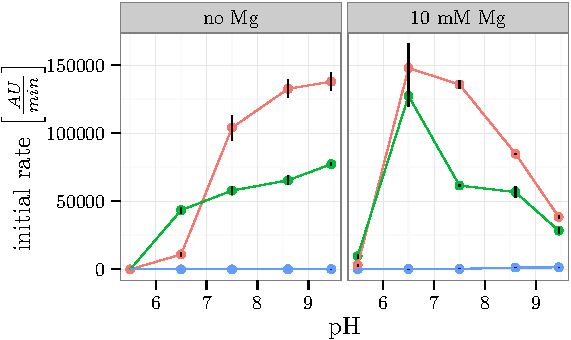
\includegraphics{analysis_tufte_files/figure-latex/unnamed-chunk-4-1.pdf}
\caption{pH-profiles for SAH production. Substrates: red -- caffeic acid, green -- eriodictyol, blue -- iso-ferulic acid}
\end{figure}

Iso-ferulic acid is no catechol, rather it bears a
(4'-O-methyl-3'-hydroxyl)-moiety. But clearly iso-ferulic acid is
methylated at higher pH values, especially when Mg is present.

\begin{marginfigure}
 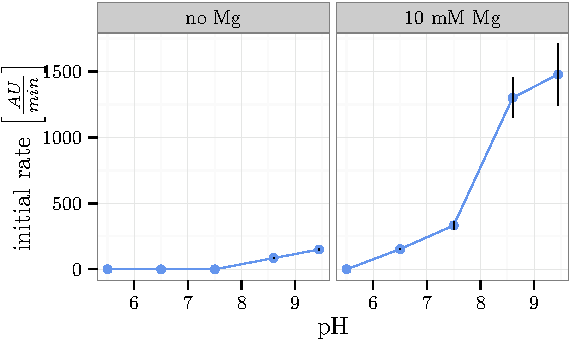
\includegraphics{analysis_tufte_files/figure-latex/unnamed-chunk-5-1.pdf}
\caption{pH-profiles for the substrate iso-ferulic acid. The reaction occurs much slower than for the catecholic substrates.}
\end{marginfigure}

\newthought{The pH-optimum} of the enzyme seems to shift to lower
pH-values with addition of Mg. When no Mg is added the initial velocity
increases with pH. However, upon Mg addition the maximum is reached at a
pH of around 6.8 for the catecholic derivatives. After that the rate
drops drastically.

\newthought{For iso-ferulic acid} this effect is not present. The rates
are much higher, when Mg is added. Even at high pH-values. When no Mg is
added there is virtually no conversion at low pH values. Thisa could
correlate with the pKa.

\subsection{Regression tree}\label{regression-tree}

\begin{figure}
 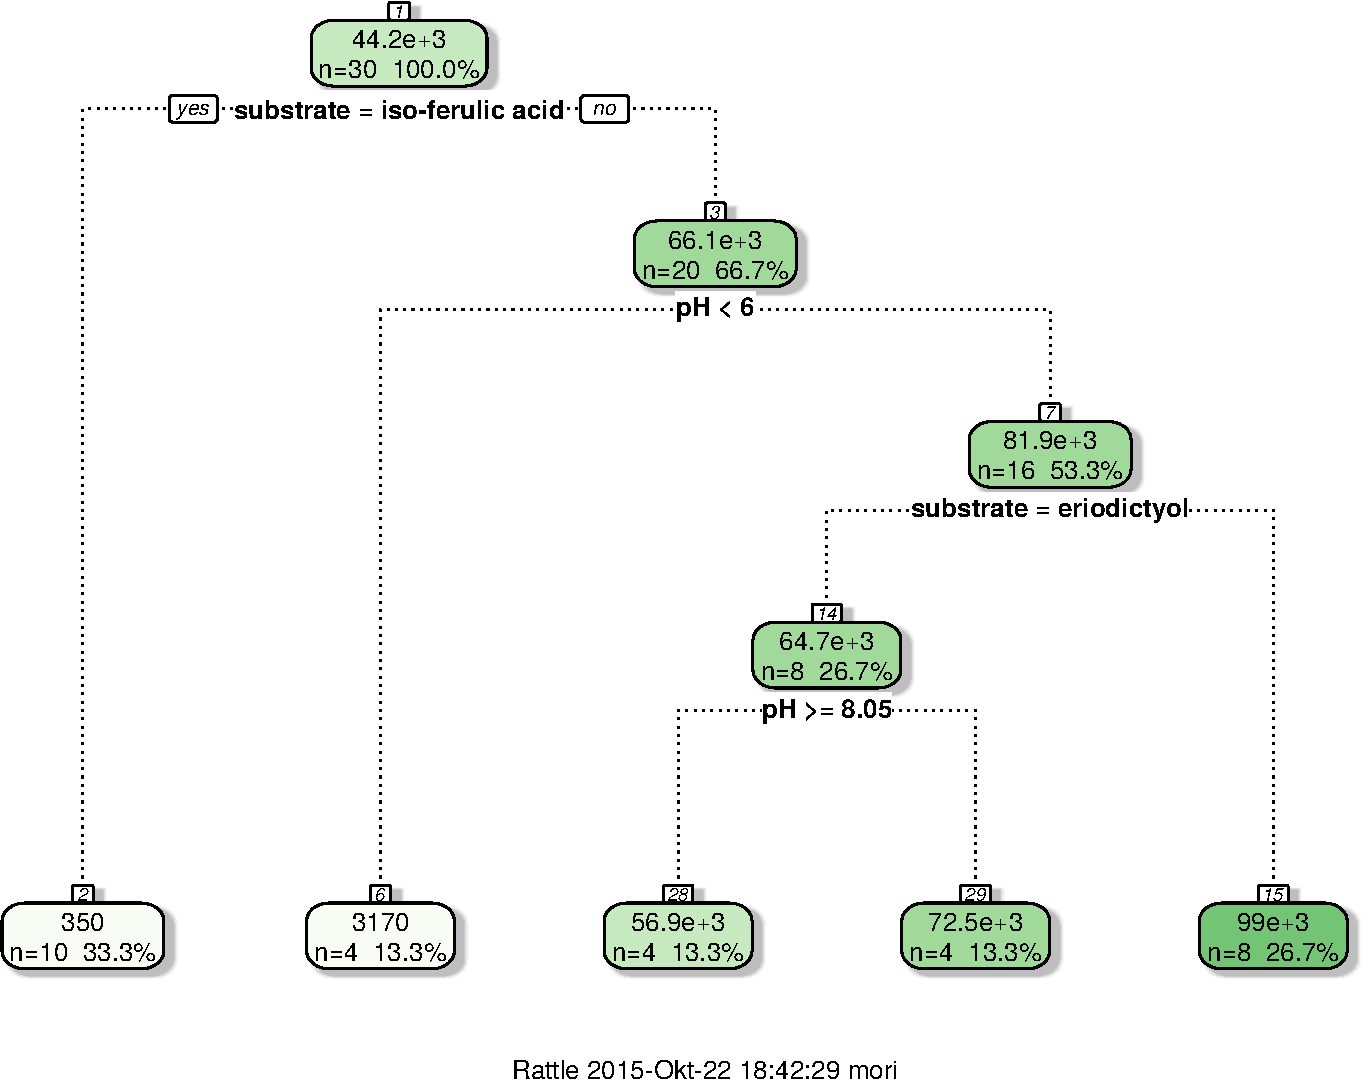
\includegraphics{analysis_tufte_files/figure-latex/unnamed-chunk-6-1.pdf}
\end{figure}

\section{Linear models}\label{linear-models}

The motif plays an important role for catalysis. Thus, the data set was
split up into two separate ones. One including only iso-ferulic acid and
one including the other two catecholic substrates.

\newthought{Enzymatic reactionsa are hard to model} using simple linear
models. This is due to the fact that enzymatic mechanisms are hardly
linear. In fact enzymatic mechanisms are highly complex and non-linear.
However for a close approximation it should do.

\subsection{Iso-ferulic acid dataset}\label{iso-ferulic-acid-dataset}

93.55\% of the variance in the data can be described by the model
\texttt{rate\textasciitilde{}pH*Mg}, including both main effects and
interaction terms. Both main effects (pH and Mg), as well as the
interaction term seem to be significant, as suggestes by their p-values
below 0.01 when compared by ANOVA. However, the model would deem the
main effect of pH not significant (p-value 0.51).

\begin{table}[ht]
\centering
\begin{tabular}{lrrrrr}
  \toprule
 & Df & Sum Sq & Mean Sq & F value & Pr($>$F) \\ 
  \midrule
pH          & 1 & 1016694.74 & 1016694.74 & 33.60 & 0.0012 \\ 
  Mg          & 1 & 918173.79 & 918173.79 & 30.34 & 0.0015 \\ 
  pH:Mg       & 1 & 699519.42 & 699519.42 & 23.12 & 0.0030 \\ 
  Residuals   & 6 & 181570.88 & 30261.81 &  &  \\ 
   \bottomrule
\end{tabular}
\caption{ANOVA-table for the simple model for iso-ferulic acid. The interaction term is included.} 
\end{table}\begin{table}[ht]
\centering
\begin{tabular}{rrrrr}
  \toprule
 & Estimate & Std. Error & t value & Pr($>$$|$t$|$) \\ 
  \midrule
(Intercept) & -241.4238 & 420.1485 & -0.57 & 0.5864 \\ 
  pH & 38.4239 & 54.9778 & 0.70 & 0.5108 \\ 
  MgTRUE & -2201.3084 & 594.1797 & -3.70 & 0.0100 \\ 
  pH:MgTRUE & 373.8131 & 77.7503 & 4.81 & 0.0030 \\ 
   \bottomrule
\end{tabular}
\caption{Model summary for the linear model (lm()).} 
\end{table}\begin{marginfigure}
 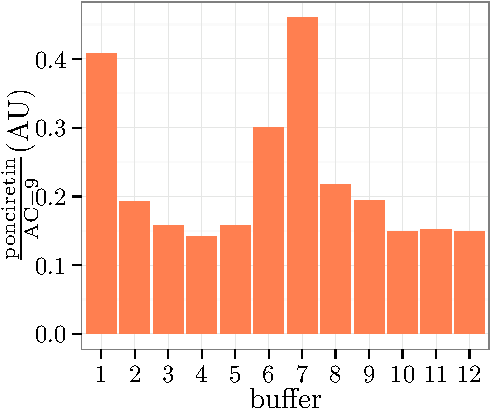
\includegraphics{analysis_tufte_files/figure-latex/unnamed-chunk-7-1.pdf}
\caption{pH profiles for iso-ferulic acid with predicted data from the model. The grey ribbon displays the 95\% prediction interval.}
\end{marginfigure}

The model predicts the data sufficiently correct. Plus it is not the
goal to make predictions, rather than draw inferences.

\subsection{Catechols dataset}\label{catechols-dataset}

The catecholic substrates were modelled accordingly. However, because
the non-linear nature of the data a quadratic term was included in the
model. The model formula was
\texttt{rate\textasciitilde{}Mg*pH+I(pH\^{}2)}. The substrate was not
inlcued in the model for the sake of simplicity, although it undoubtetly
has an influence.

\begin{table}[ht]
\centering
\begin{tabular}{lrrrrr}
  \toprule
 & Df & Sum Sq & Mean Sq & F value & Pr($>$F) \\ 
  \midrule
Mg          & 1 & 207399999.37 & 207399999.37 & 0.19 & 0.6695 \\ 
  pH          & 1 & 7699725667.36 & 7699725667.36 & 7.06 & 0.0188 \\ 
  I(pH\verb|^|2)     & 1 & 11409722262.76 & 11409722262.76 & 10.46 & 0.0060 \\ 
  Mg:pH       & 1 & 8909537802.01 & 8909537802.01 & 8.17 & 0.0127 \\ 
  Mg:I(pH\verb|^|2)  & 1 & 5057251759.85 & 5057251759.85 & 4.64 & 0.0492 \\ 
  Residuals   & 14 & 15273527656.71 & 1090966261.19 &  &  \\ 
   \bottomrule
\end{tabular}
\caption{ANOVA-table for the simple model foir iso-ferulic acid. The interaction term is included.} 
\end{table}\begin{table}[ht]
\centering
\begin{tabular}{rrrrr}
  \toprule
 & Estimate & Std. Error & t value & Pr($>$$|$t$|$) \\ 
  \midrule
(Intercept) & -421929.9946 & 356063.7085 & -1.18 & 0.2557 \\ 
  MgTRUE & -839999.8874 & 503550.1257 & -1.67 & 0.1175 \\ 
  pH & 103271.3345 & 97739.1728 & 1.06 & 0.3086 \\ 
  I(pH\verb|^|2) & -4977.7406 & 6512.6996 & -0.76 & 0.4574 \\ 
  MgTRUE:pH & 266920.7964 & 138224.0638 & 1.93 & 0.0740 \\ 
  MgTRUE:I(pH\verb|^|2) & -19830.2264 & 9210.3481 & -2.15 & 0.0492 \\ 
   \bottomrule
\end{tabular}
\caption{Model summary for the linear model (lm()).} 
\end{table}\begin{marginfigure}
 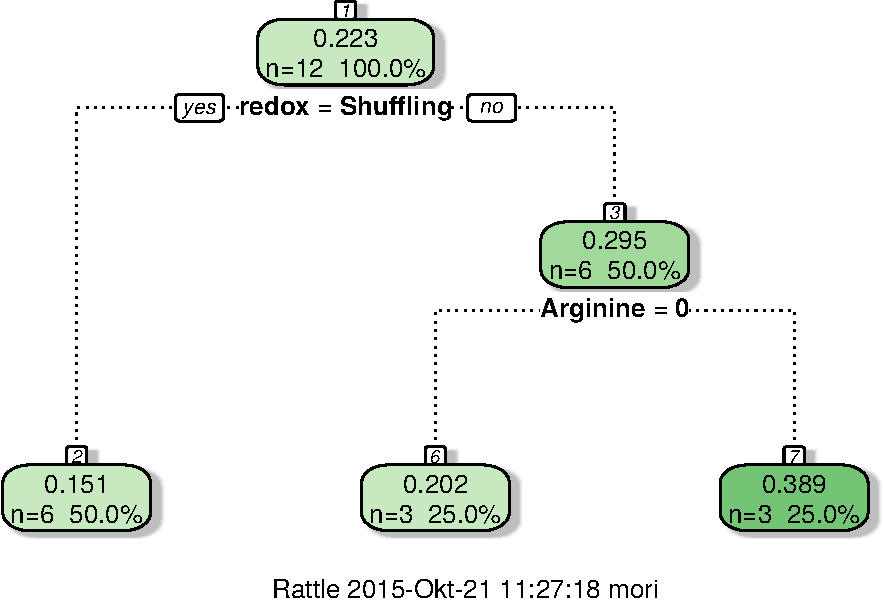
\includegraphics{analysis_tufte_files/figure-latex/unnamed-chunk-8-1.pdf}
\caption{pH profiles for catecholic substrates with predictions and 95\% prediction interval.}
\end{marginfigure}

\newthought{The trend of the curve} is described by the model
sufficiently correct. Together with the data from the ANOVA table, it
can be concluded that there is an interaction effect between pH and Mg.
However, the linear model is hardly sufficient to predict the correct
curve. In fact it merely accounts for 68\% of the variance
(R\textsuperscript{2}=0.6855).

\section{Cross validation lasso
regression}\label{cross-validation-lasso-regression}

The split datasets were also modelled using lasso regression, together
with a cross validation approach.

\subsection{CV lasso on iso-ferulic
acid}\label{cv-lasso-on-iso-ferulic-acid}

Since only non-zero coefficients are shown, it can also be concluded
here that pH and Mg display both main and an interaction effect for
iso-ferulic acid. Diagnostic plots that show the optimization for the
tuning parameter lambda are displayed on the margin. The final shrunken
model includes only three variables (Mg, pH and Mg:pH interaction).

\begin{marginfigure}
 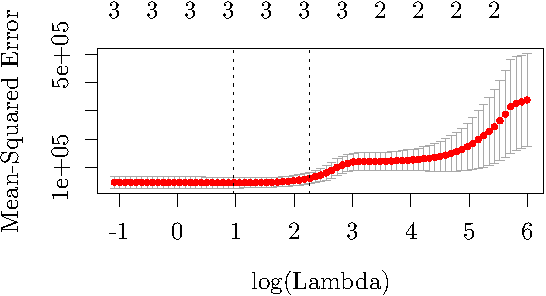
\includegraphics{analysis_tufte_files/figure-latex/unnamed-chunk-9-1.pdf}
\end{marginfigure}\begin{marginfigure}
 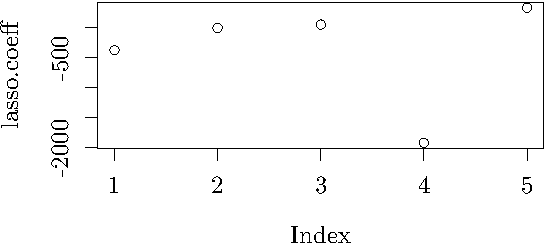
\includegraphics{analysis_tufte_files/figure-latex/unnamed-chunk-9-2.pdf}
\end{marginfigure}\begin{marginfigure}
 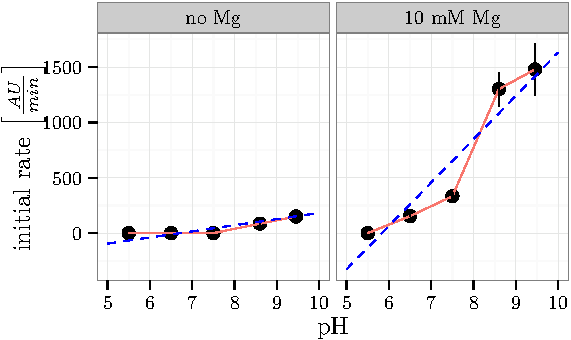
\includegraphics{analysis_tufte_files/figure-latex/unnamed-chunk-9-3.pdf}
\end{marginfigure}

\begin{margintable}
\centering
\begin{tabular}{rlr}
  \toprule
 & variable & coefficient \\ 
  \midrule
1 & (Intercept) & -371.3745 \\ 
  2 & pH & 55.3578 \\ 
  3 & MgTRUE & -1913.8456 \\ 
  4 & pH:MgTRUE & 336.2752 \\ 
   \bottomrule
\end{tabular}
\caption{Variables and coefficients that were retained. Non-zero coefficients not shown.} 
\end{margintable}

\newpage

\subsection{CV lasso on catechols}\label{cv-lasso-on-catechols}

The same CV method was also applied for the catecholic substrate data.
The model formular was \texttt{rate\textasciitilde{}pH*Mg*I(pH\^{}2)}.
After shrinkage the model still contained a lot of factors. All the main
effects, as well as 2 two-way interaction and one 3-way interaction
effect. This makes the model very complex. However from the predicted
curves it is clear that the model roughly describes the data. This can
be seen as evidence that the relationhsip of pH and rate includes a
quadratic term.

\begin{marginfigure}
 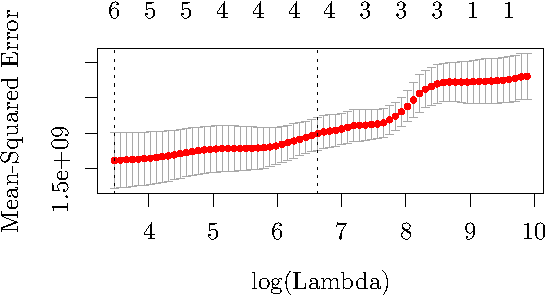
\includegraphics{analysis_tufte_files/figure-latex/unnamed-chunk-11-1.pdf}
\end{marginfigure}\begin{marginfigure}
 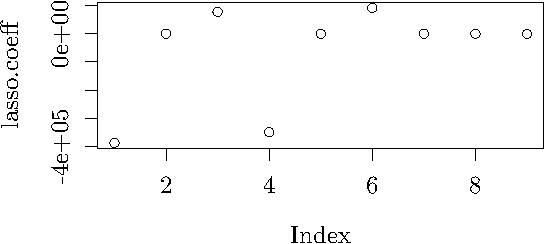
\includegraphics{analysis_tufte_files/figure-latex/unnamed-chunk-11-2.pdf}
\end{marginfigure}\begin{marginfigure}
 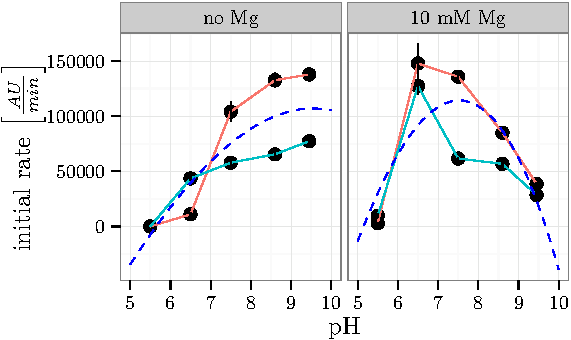
\includegraphics{analysis_tufte_files/figure-latex/unnamed-chunk-11-3.pdf}
\end{marginfigure}

\begin{margintable}
\centering
\begin{tabular}{rlr}
  \toprule
 & variable & coefficient \\ 
  \midrule
1 & (Intercept) & -387606.9260 \\ 
  2 & pH & 77725.3554 \\ 
  3 & MgTRUE & -349735.8685 \\ 
  4 & I(pH\verb|^|2) & -0.0045 \\ 
  5 & pH:MgTRUE & 92049.1328 \\ 
  6 & pH:I(pH\verb|^|2) & -284.3251 \\ 
  7 & pH:MgTRUE:I(pH\verb|^|2) & -715.0114 \\ 
   \bottomrule
\end{tabular}
\caption{Variables and coefficients that were retained. Non-zero coefficients not shown.} 
\end{margintable}

\section{Conclusion}\label{conclusion}

\begin{itemize}
\itemsep1pt\parskip0pt\parsep0pt
\item
  big difdference in rate of catecholic and non-catecholic substrates
\item
  rate is influenced by pH, Mg
\item
  pH and Mg have interaction effect
\item
  pH/rate relationship includes a quadratic term \(\rightarrow\) common
  form for pH-profles of enzymes
\item
  Mg addition shifts pH optimum of enzyme to pH around 7 for catechols
\item
  Mg addition is beneficial for conversion of iso-ferulic acid
\end{itemize}

\section{Specific activity}\label{specific-activity}

The specific activity can be calculated. Therefore we approximate that
the molar extinction coefficient for SAM and SAH are the same and the
combined area-under-the-curve (AUC) of the SAM and SAH peak are 100\% of
substrate or 500 uM. The concentration for either one of SAM or SAH can
then be estimated from that relationship.

\begin{marginfigure}
$$A_\mathrm{SAM} + A_\mathrm{SAM} = 1 \approx 500 \mathrm{uM}$$
$$x_\mathrm{SAH} = \frac{A_\mathrm{SAH}}{A_\mathrm{SAM} + A_\mathrm{SAM}}$$
$$c_\mathrm{SAH} = x_\mathrm{SAH} \times 500 \mathrm{uM}$$
$$n_\mathrm{SAH} = c_\mathrm{SAH} \times V^\mathrm{inject}$$
\caption{Calculation of specific activity.}
\end{marginfigure}

From the concentration and the injection volume (10 uL) the amount
(moles) of substrate or product can be estimated. From that the specific
activity can be calculated from the slope of the P-t-diagram and the
amount of enzyme used (0.2 ug/uL). First the above equations were
employed to calculate the concentration of SAH and SAM in each sample.
This was plotted against the area. The curve displays a linear
relationship, although the errors seem to get larger with increasing
area. The errors seem to be non-normally distributed. However as a rough
estimation is will suffice.

The data for each SAH and SAM were fitted with alinear model
\texttt{concentration\textasciitilde{}area}.

\begin{equation}
c = \mathrm{a}\times A + \mathrm{b}
\end{equation}

For SAH the values for a and b were 1.272e-04 and 6.219e-02
respectively.

\begin{marginfigure}
 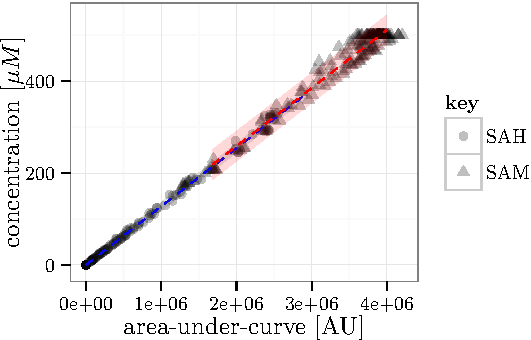
\includegraphics{analysis_tufte_files/figure-latex/unnamed-chunk-13-1.pdf}
\caption{The calculated concentrations from the areas. The error looks as though it is not normally distributed.}
\end{marginfigure}\begin{table}[ht]
\centering
\begin{tabular}{rrrrr}
  \toprule
 & Estimate & Std. Error & t value & Pr($>$$|$t$|$) \\ 
  \midrule
(Intercept) & 0.0622 & 0.4018 & 0.15 & 0.8772 \\ 
  area & 0.0001 & 0.0000 & 292.71 & 0.0000 \\ 
   \bottomrule
\end{tabular}
\caption{Linear fit for SAH area and concentration.} 
\end{table}\begin{table}[ht]
\centering
\begin{tabular}{rrrrll}
  \toprule
 & max.U.mg & max.pkat.mg & at.pH & substrate & Mg \\ 
  \midrule
1 & 49.42 & 823.73 & 9.45 & eriodictyol & FALSE \\ 
  2 & 81.26 & 1354.41 & 6.50 & eriodictyol & TRUE \\ 
  3 & 0.41 & 6.78 & 9.45 & iso-ferulic acid & FALSE \\ 
  4 & 1.25 & 20.85 & 9.45 & iso-ferulic acid & TRUE \\ 
  5 & 87.96 & 1465.93 & 9.45 & caffeic acid & FALSE \\ 
  6 & 94.30 & 1571.61 & 6.50 & caffeic acid & TRUE \\ 
   \bottomrule
\end{tabular}
\caption{The maximal activities obtained for each sample (substrate/Mg combination). Activities are given in nmol min\textsuperscript{-1} mg\textsuperscript{-1}} 
\end{table}

The maximum enzyme activities that were calculated here are comparable
to the ones that were obtained previously (DIM paper PFOMT, wt(caffeic
acid) \(\approx\) 72 nmol min\textsuperscript{-1}
mg\textsuperscript{-1}, Vogt (2003) nativ(6-OH-kaempferol) \(\approx\)
830 pkat per mg).

\begin{marginfigure}
 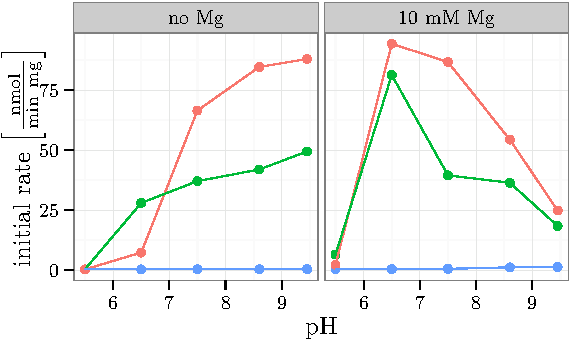
\includegraphics{analysis_tufte_files/figure-latex/unnamed-chunk-14-1.pdf}
\caption{pH-profiles with specific activities.}
\end{marginfigure}\begin{marginfigure}
 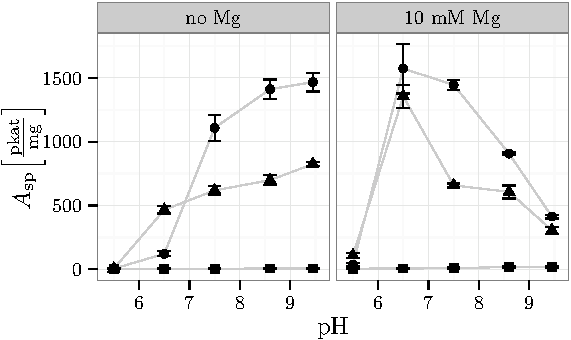
\includegraphics{analysis_tufte_files/figure-latex/unnamed-chunk-14-2.pdf}
\caption{pH-profiles with specific activities.}
\end{marginfigure}


\end{document}
